% AER-Article.tex for AEA last revised 22 June 2011
\documentclass[AER,draftmode]{AEA}

\usepackage{graphicx}
\usepackage{apacite}
\usepackage[colorinlistoftodos]{todonotes}

\usepackage{setspace}


% The mathtime package uses a Times font instead of Computer Modern.
% Uncomment the line below if you wish to use the mathtime package:
%\usepackage[cmbold]{mathtime}
% Note that miktex, by default, configures the mathtime package to use commercial fonts
% which you may not have. If you would like to use mathtime but you are seeing error
% messages about missing fonts (mtex.pfb, mtsy.pfb, or rmtmi.pfb) then please see
% the technical support document at http://www.aeaweb.org/templates/technical_support.pdf
% for instructions on fixing this problem.

% Note: you may use either harvard or natbib (but not both) to provide a wider
% variety of citation commands than latex supports natively. See below.

% Uncomment the next line to use the natbib package with bibtex 
%\usepackage{natbib}

% Uncomment the next line to use the harvard package with bibtex
%\usepackage[abbr]{harvard}

% This command determines the leading (vertical space between lines) in draft mode
% with 1.5 corresponding to "double" spacing.
\draftSpacing{1.5}
\setlength{\marginparwidth}{4cm}

\begin{document}

\title{Does Coverage of Sexual Assault Cases Ease the Reporting Decision? Evidence from FBI Data}
\shortTitle{Sexual Assault Reporting}
\author{Harry Elworthy\thanks{Duke University, 837 Clarendon St Durham NC, harryelworthy@gmail.com.}}
\date{\today}
\pubMonth{}
\pubYear{}
\pubVolume{}
\pubIssue{}
\JEL{}
\Keywords{}

\begin{abstract}
Your abstract here.

Files available at \url{github.com/harryelworthy/Thesis}
\end{abstract}


\maketitle

%American Economic Review Pointers:

%\begin{itemize}
%\item Do not use an "Introduction" heading. Begin your introductory material
%before the first section heading.

%\item Avoid style markup (except sparingly for emphasis).

%\item Avoid using explicit vertical or horizontal space.

%\item Captions are short and go below figures but above tables.

%\item The tablenotes or figurenotes environments may be used below tables
%or figures, respectively, as demonstrated below.

%\item If you have difficulties with the mathtime package, adjust the package
%options appropriately for your platform. If you can't get it to work, just
%remove the package or see our technical support document online (please
%refer to the author instructions).

%\item If you are using an appendix, it goes last, after the bibliography.
%Use regular section headings to make the appendix headings.

%\item If you are not using an appendix, you may delete the appendix command
%and sample appendix section heading.

%\item Either the natbib package or the harvard package may be used with bibtex.
%To include one of these packages, uncomment the appropriate usepackage command
%above. Note: you can't use both packages at once or compile-time errors will result.

%\end{itemize}

\clearpage
Approximately 20\% of women in the United States are sexually assaulted at some point in their lives, with more than a third of these assaults occurring before the victim turns 18 \cite{black_national_2011}. Approximately 20\% to 25\% of women nationally are sexually assaulted at some point during their college careers \cite{fisher_sexual_2000}. At Duke, this figure is estimated at closer to 40\%, as well as 10\% of men \cite{fox_university_2017} \todo{I can sort these statistics better to tell a better story. I also should note male victims earlier.}. Despite this, few assaults are reported to police or to other authorities such as universities, for a number of reasons, including self-blame or guilt, fear of the perpetrator or fear of not being believed \cite{du_mont_role_2003}. A number of different measures have been taken by many schools to address campus sexual assault, including significant federal reform via Title IX reform in 2011, which affected almost every school in the US. These changes aimed to make reporting easier for an assault victim, thus increasing reports and hopefully, in equilibrium, decreasing assault.

The issue of non-reporting has been especially salient over the past years, as first Harvey Weinstein, then Supreme Court nominee - now Justice - Brett Kavanaugh made national headlines being accused of sexual assaults that were not reported to police at the time they were committed \todo{Not completely sure this the case for Weinstein}. President Trump tweeted in response to the Kavanaugh claims: "I have no doubt that, if the attack on Dr. Ford was as bad as she says, charges would have been immediately filed with local Law Enforcement Authorities by either her or her loving parents" \citeyear{trump_i_2018}. As above, there are many reasons why an individual may not report: social pressures, abusive relationships, and fear of not being believed, for example. More importantly, however, this tweet illustrates a source of motivation for this paper: had Dr. Ford reported when the crime had been committed, her testimony now would be more impervious to detractors. There are many reasons that increased reporting would be a desirable outcome - this is just one of them. \todo{Need more on why reporting is desirable}

The #metoo movement that the Weinstein allegations started focused on women coming forward with their sexual assault stories because they saw others come forward with theirs - thus the 'me too.' This idea highlights an important question: are victims of sexual assault encouraged to report to police or other authorities by coverage of other victims reporting? Several other questions follow: if they are encouraged, what is the magnitude in the increase in reports? How long does the increase in reporting last for? How does local reporting affect reporting vs. national reporting? And - most importantly - does this coverage affect the behavior of potential perpetrators?

In this paper, I explore these questions using incident-level FBI data of crime reports from 1991 to 2016, along with data from Google Trends. I also conduct a number of event studies using Title IX investigations of universities and a novel dataset of high-profile sexual assault allegations. 

\section{Background}

The background section of \cite{lindo_college_2018} has a good background on sexual assault reporting, as do a number of my cited papers. I need to make my own ASAP! I've deleted all previously written stuff as my paper has pivoted away from it enough to make it pretty irrelevant. Here's what I'd like to talk about in my background section when I write it:

\begin{itemize}
    \item One or two sentences about the multitude of work on prostitution/porn/sexual harrassment etc. by economists in the past two decades (many of the pieces in my Lit Review are like this)
    \item Background on history of economic papers on sexual assault reporting decision (\citeA{allen_reporting_2007} needs to be much more at the fore). 
    \item Papers from other disciplines on the reporting decision - more research needs to be done here. Psychology/sociology. Would be good for talking about cost of reporting later.
    \item Short history of high profile sexual assault cases. Run through most important ones from my list of events since 2008, plus some discussion of pre-2008.
    \item Some on #metoo? Although not directly relevant to my investigation as such
    \item Much more on why reporting is so important - in itself and in what we hope to see in its outcomes, i.e. less assaults
\end{itemize}

I'd also like to include something like Figure~\ref{figure:police_yearly} below. Note that this is not a great graph right now, as it shows a time when the number of police stations reporting these numbers was increasing. I need to make it per-capita, which will just take a re-jigging of my code that runs on the server. 

\begin{figure}

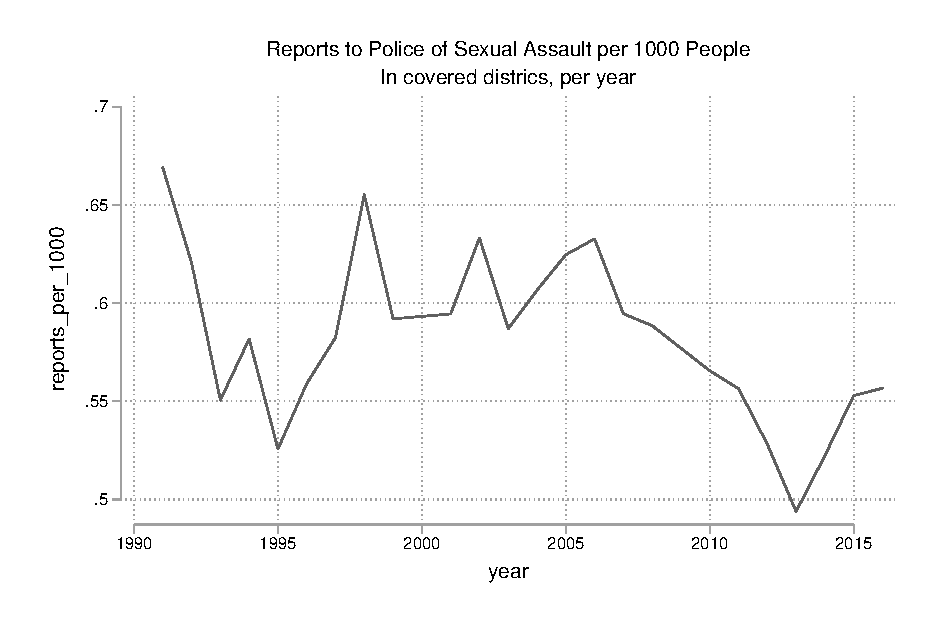
\includegraphics[width=\linewidth]{figures/police_yearly_reports.eps}

\caption{Reports to Police per Person, 1991 to 2015} \label{figure:police_yearly}
\end{figure}

\todo{Unsure why all my figures have big black bar on the right? Need to fix!}

This is obviously a big area of work for my paper. My literature review is also still (I know I know) not organized at all around my paper, and is instead just a list of summaries. This is also a big area of work. Because I've been shifting my research question around, some of these are now irrelevant while others have become much more important. This week my big task will be synthesizing the intro, my background and the lit review into one coherent package.

\section{Literature Review}
\todo{This is unchanged from last time.}
Since Becker outlined his economic model of crime, illicit activities have continued to have a place in the economic literature. Sexual assault has received a share of this attention, although perhaps less so than other crimes. One reason for this deficit is the difficulty of gathering accurate data on sexual assault. Crime is underreported in general, sexual assault especially \cite{kilpatrick_drug-facilitated_2007} \cite{fisher_sexual_2000}. Recently, however, several economics papers have focused on sexual assault and harassment. 

\citeA{allen_reporting_2007} investigates the factors that influence an individual's decision to report a rape to law enforcement using survey data from The National Sample of Rape Victims, completed in 1985 and released in 2000, and finds that victims will be more likely to report sexual assault given more 'social support and ancillary evidence associated with the crime.' This paper is important to this investigation as it shows that the decision to report is influenced by factors that may be affected by policy, and thus supports the notion that policy to ease the reporting process could be beneficial. It is also some of the only research done on what affects the individual's decision to report. Given that I will be diving deeper into reasons this decision may have been made more often after 2011, this seems especially important to my investigation.

\citeA{yung_concealing_2015} investigates the idea that universities undercount reports in order to save face.  Comparing report numbers from years before and after an audit by the OCR, the paper estimates a consistent 40\% uptick in reports by universities in the year of an audit, followed by a return to preexisting trends the year directly after an audit. This is relevant for my paper, as this undercounting could affect the accuracy of the CSS data I am using, although the homogeneity found in undercounting indicates that it should not lead to bad estimates.

\citeA{lindo_college_2018} looks at the effect of partying culture on reports of sexual assault. Specifically, using the plausible exogeneity of Division 1 football games, the paper estimates the effects of increased partying that comes with such events on reports of rape to law enforcement. The authors find a 28\% increase in rape reports associated with game days. Estimates are higher when the opponent is a rival, when the game is a Home rather than Away game, and when the game is televised. This paper is useful as it is a recent, high profile economics paper on the causes of sexual assault on college campuses, and for its use of NBIRS data, which will allow my paper to make use of this data much more easily.

\citeA{lindo_any_2018} considers the effects of a Title IX investigation on a universities outcomes such as enrolment, applications, degree completion and donations. Their estimates show significant upticks in both enrolment and applications following an investigation for both men and women\todo{Would be interesting to do this and see if the size of a school's increase in Reports has any effect on the size of the increase in enrollment}, with no evidence of effects on degree completion or donations. As part of their analysis, they use Google Trends data as a proxy for public awareness of investigations, concluding that the investigations are indeed in the public spotlight, even while federal policy on sexual assault may not be. The paper has an in-depth background of the 2011 Title IX changes that is very useful for my paper, as well as being closely related in subject. 

\section{Data Summary}

I have four main data sources for this project: \todo{Need to include sources for these, make this not a bullet point list, explain them a bit more in detail (I use on-campus reports etc.) but will wait to see how much I use school data in the end for this.}
\begin{itemize}
    \item National Incident-Based Reporting System (NIBRS) Data
    \begin{itemize}
        \item Individual reports of crime to police stations. 1991 to 2016.
        \item About 40\% of population covered (some police stations don’t report) and this number has increased since 1991 as more stations have begun reporting.
        \item Timestamped, both report and incident datetime, lots of auxiliary information i.e. about the victim in question
        \item Because is by incident, can be collapsed to any specification: Nationally Daily, State-by-Week, etc. 
    \end{itemize}
    \item Google Trends data
    \begin{itemize}
        \item Daily and weekly trends for “sexual assault” 2008 to 2018 \footnote{Decided on "sexual assault" as "rape" tended to have a lot of unsavoury related searches, mostly pornography related, whereas searches for sexual assault tended to be related to cases of sexual assault. I test both for salience, and "rape" is not responsive to Title IX cases while "sexual assault" is. May try to add both back in.} \todo{Can probably change this to 2004 as not using News, need to rerun}
        \item National and statewide trends.
        \item Relative trends out of 100, scaled to 2008 numbers, so some numbers later on are higher.
        \item Merge daily with police data for most of my investigation. Thus have reports of sexual assault grouped by either report or incident date together with Google Trends, daily, from 2008 to 2016. 
    \end{itemize}
    \item Related Events with Prominent News Coverage
    \begin{itemize}
        \item This is very recent, I need to go over it with my advisor etc, but I think it is useful. 
        \item I've created a dataset of 35 big-headline sexual assault events from 2008 until 2016, along with the dates that they were first in the news.
        \item To do this I used Google's Related Topics tool. This tool shows for a given time period what related searches were to a given search.
        \item I looked at related search terms to 'sexual assault' each day that the trend for 'sexual assault' was above 70\% of its 6 month maximum. For events that had coverage for multiple days, I only included the first day. If there was more than a month between coverage I counted these as separate events. 
        \item The 35 events I found are shown in Appendix 1. I also categorize them into allegations and 'big allegations,' which are events that held the google trend above 75 for more than 3 days in a row. 
        \item I am sure that I've missed some events as my process could have been better, but each of these events is definitely a high profile sexual assault event. For an event study, it would definitely be better to get more events, but my results should be relatively good estimators as is (just with large standard errors from low n)
    \end{itemize}
    \item Campus Safety and Security (CSS) Data
    \begin{itemize}
        \item Collected and distributed by the Department of Education, 2005 to 2016
        \item Reports of Sexual Assault by year by university, for all schools that receive financial aid (7663 schools that span the full time period)
        \item Not granular at all - because of an internal standards change in 2013 for how to count sexual assault reports, have to include all assaults, including non-forcible ones/statutory assault/etc.
        \item Can tie in a lot of auxiliary data by school ID from other sources, such as funding, SAT scores, enrollment by race/sex, etc.
    \end{itemize}
    \item Title IX Cases
    \begin{itemize}
        \item Opened when a student believes they were mistreated by a school's reporting system
        \item Only began after 2011
        \item Data for each start/end date by school
        \item Used in \citeA{lindo_any_2018} to test effects on enrollment/applications/etc. They find increase in these factors, not decrease, even for women. They also find that case opening has sizable impact on google trends for “[school name] rape” – so somewhat salient. I hope to expand this salience check.
        \item I am basing my panel data models off of theirs'
    \end{itemize}
\end{itemize}

This section needs to be taken out of bullet form once I've settled on my final list of figures and tables. I'd also like to have a table of summary statistics here.

\section{Methodology}

In the first half of this section I'll discuss sexual assault, both the crime and the reporting of it, from an economic standpoint. This is outlined below. Second half, I outline the regression equations I'll be using.

\begin{itemize}
    \item Discussion of why someone might not report, fueled by \citeA{allen_reporting_2007} (where we see that a social safety net helps ease the reporting decision among other things) and \citeA{du_mont_role_2003} as well as any other papers I find about this
    \item Pull that discussion into a more formal discussion of the costs and uncertainty that one faces in reporting, and how coverage of sexual assault might affect that in one way or another: by lowering or raising expected cost of social stigma, by inspiring and perhaps increasing expected benefit, the idea that reporting can help reduce sexual assault. More here, need to come up with as exhaustive a list as I can, as this is important.
    \item Then spend some time discussing a similar thing but for potential perpetators - expected cost of assault. Obviously even more than the other one this is a behaviour that is tough to rationalize, but it's not wild to think (and one would seriously hope) that at the margin these people can be influenced one way or another
    \item Talk about the two in tandem, and again why hopefully reporting affects the second, and thus is important. If possible, this link would be great to try to estimate, but very difficult given the nature of the data. 
\end{itemize}

In this paper, I'll run a number of time-series, panel-data and event-study type regressions. The general form of these regression equations is outlined below. My time-series regressions are at the daily level, and are of the form: 

$$ 
y_{t} = \beta_{0} + \sum_{b=-7}^{7} \delta_{b} x_{t+b} + \gamma_{t} + \varepsilon_{t}
$$

Where $y_{t}$ is the outcome variable in question; $x_{t+b}$ is the independent variable in question along with a set of leads and lags, and $\gamma{t}$ is a vector including day-of-week, week-of-year and year fixed-effects. These fixed effects should take care of most seasonality in the data. \todo{I need to decide on a good reason for how many leads and lags I will be including, then put this reasoning here. Advisor also said that in final form, i.e. for tables rather than graphing, I should drop leads from this.}

My panel data regressions are of the form:

$$ 
y_{i,t} = \beta_{0} + \sum_{b=-7}^{7} \delta_{b} x_{i,t+b} + \alpha_{i} + \gamma_{t} + \varepsilon_{i,t}
$$

Where $y_{i,t}$ is the outcome variable in question; $x_{i,t+b}$ is the independent variable in question along with a set of leads and lags, $\alpha_{i}$ is a fixed effect at the level of the panel, usually by state or by school, and $\gamma{t}$ is a vector including year fixed-effects, as well as day-of-week and week-of-year fixed effects if the data is at the daily level.

My event study regressions are of the form:

$$ 
y_{t} = \beta_{0} + \sum_{b=-7}^{7} \delta_{b} x_{t+b} + \gamma_{t} + \varepsilon_{t}
$$

Where $y_{t}$ is the outcome variable in question; $x_{t+b}$ is a dummy for the event in question along with a set of leads and lags, and $\gamma{t}$ is a vector including day-of-week, week-of-year and year fixed-effects.

\section{Results}

\todo{I think this could maybe be split into primary and secondary results, or 'evidence from schools' or something, but need to work out narrative better first}

In general, I may drop uninteresting things from this section as I decide exactly on the narrative on my paper. I'll also include more tables in the final paper (and probably less graphs) but graphs are just nicer to glance through.

I begin by running a time-series regression of reports of sexual assault to the FBI by report-date on national Google Trends for 'sexual assault'. The results of this are shown in Figure~\ref{figure:police_trends_daily}

\begin{figure}
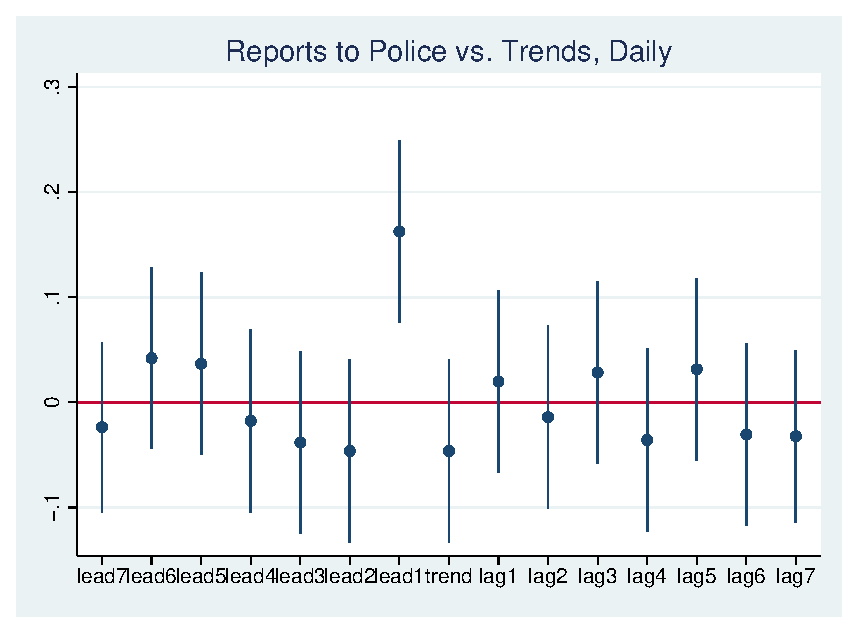
\includegraphics[width=\linewidth]{figures/police_trend_daily.eps}
\caption{Time-Series Regression of FBI Reports of Sexual Assault on Google Trends for 'sexual assault'} \label{figure:police_trends_daily}
\end{figure}

There is a clear, statistically significant effect on the first lead variable. \todo{I think I worked out that I had miscoded this, and that it was on the first lag variable. Need to go over and fix. Also fix x axis.} I discuss interpretations of the effect magnitude below. \todo{Don't actually show below yet. Probably use the Bill Cosby case as it's within sample, maybe also with a smaller case, as well as all 35 of my events. Show their graphs, eyeball approximate estimates, for the full 35 event sample calculate average effect.}

This increase in reporting is driven by reporters under 20, as shown in Figure~\ref{figure:police_trends_daily_by_age}:

\begin{figure}
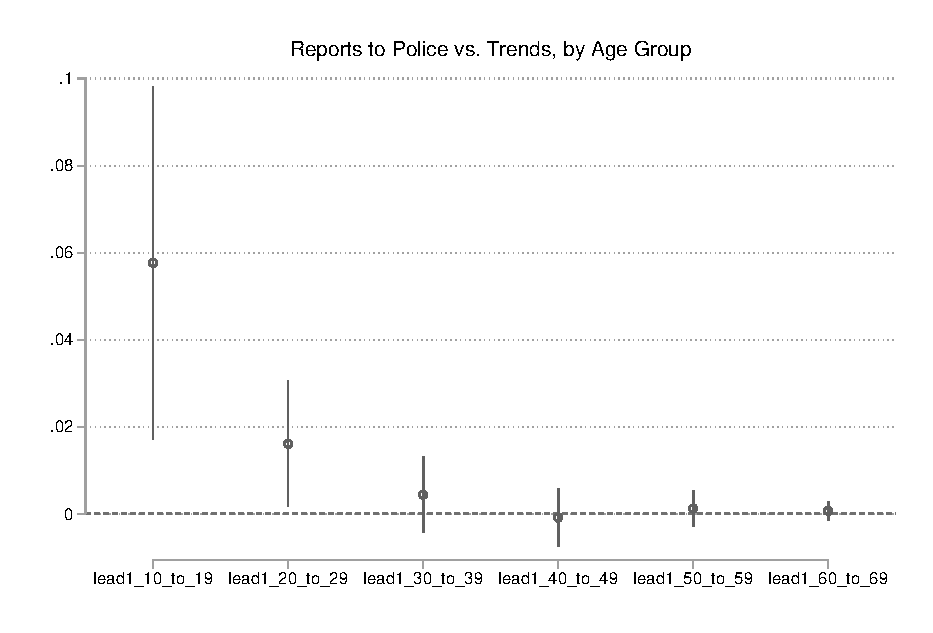
\includegraphics[width=\linewidth]{figures/police_trend_daily_agegroup.eps}
\caption{Estimates of effects of Google Trends on FBI reports of sexual assault by age group} \label{figure:police_trends_daily_by_age}
\end{figure}

\todo{Lots of x axes are bad, this is especially so. Groups are in 10 year chunks, first is 10 to 20.}

Here I'd look at how state by state variation in trends impacts reporting across states, but that regression has been giving me grief and is not presentable. I think it's going to be a small or 0 effect.

I now turn to an event study of 35 high-profile sexual-assault related stories from 2008 to 2016. To check that these events were indeed high-profile, I run an event-study regression of Google Trends on each of these event dates, results shown in Figure~\ref{figure:events_trend}:

\begin{figure}
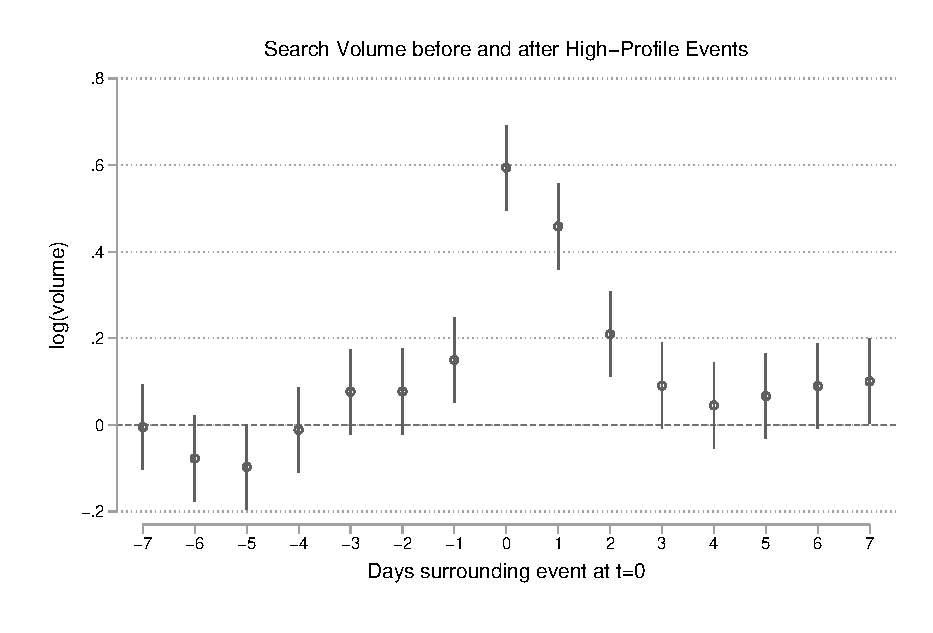
\includegraphics[width=\linewidth]{figures/events_trend.eps}
\caption{Google Trends before and after High Profile Events} \label{figure:events_trend}
\end{figure}

As can be seen, these events have sizable effects on the google trend for sexual assault that last for about 3 days. Thus they look to be good examples of random positive shocks to the google trend. \todo{Should explain this more}

I now look at the effects these events have on reports to the FBI. The results of a simple event-study regression are shown in Figure~\ref{figure:events_police}:

\begin{figure}
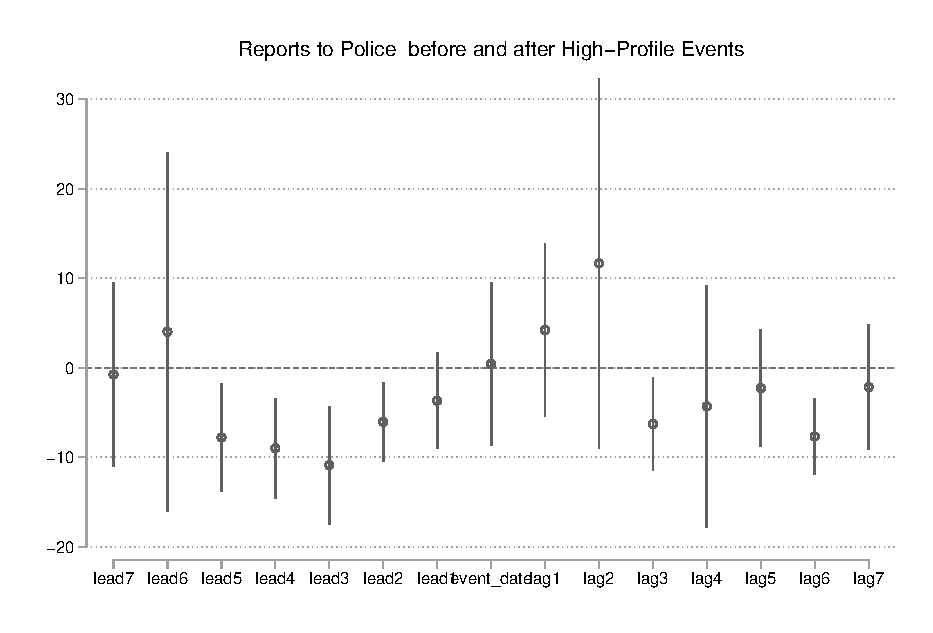
\includegraphics[width=\linewidth]{figures/events_police.eps}
\caption{Reports to the FBI before and after High Profile Events} \label{figure:events_police}
\end{figure}

There looks to be a possible effect, but it's not showing as significant on any individual day. To try to fix this, I bin the results in 3 day groups (from the 3 days that they impact google trends) in an effort to reduce standard errors. Results are shown in Figure~\ref{figure:events_police_binned}:

\begin{figure}
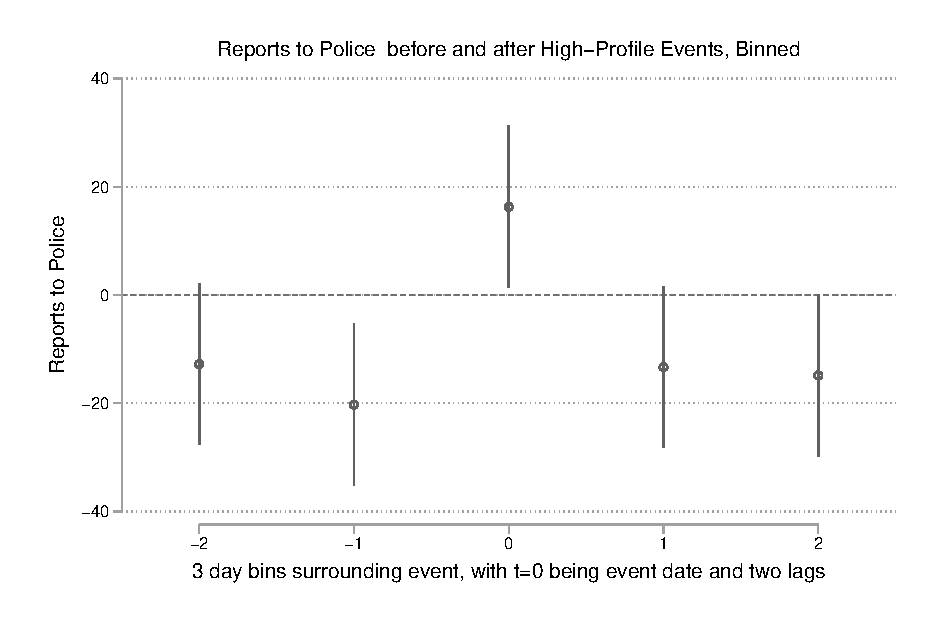
\includegraphics[width=\linewidth]{figures/events_police_binned.eps}
\caption{Reports to the FBI before and after High Profile Events, Binned} \label{figure:events_police_binned}
\end{figure}

There is still not a significant coefficient (p value is 0.15). I need to think about this and maybe bin more. Regardless, we have what looks to be a positive coefficient but SE's that are too large to confirm it. More events (higher n) would help with this.

I also estimate the effects of just events related to sexual assault allegations in Figure~\ref{figure:events_police_binned_alle}, and the effects of 'big allegations' in Figure~\ref{figure:events_police_binned_big}. Both of these figures are in 3-day bins to get consistent effect estimates.

\begin{figure}
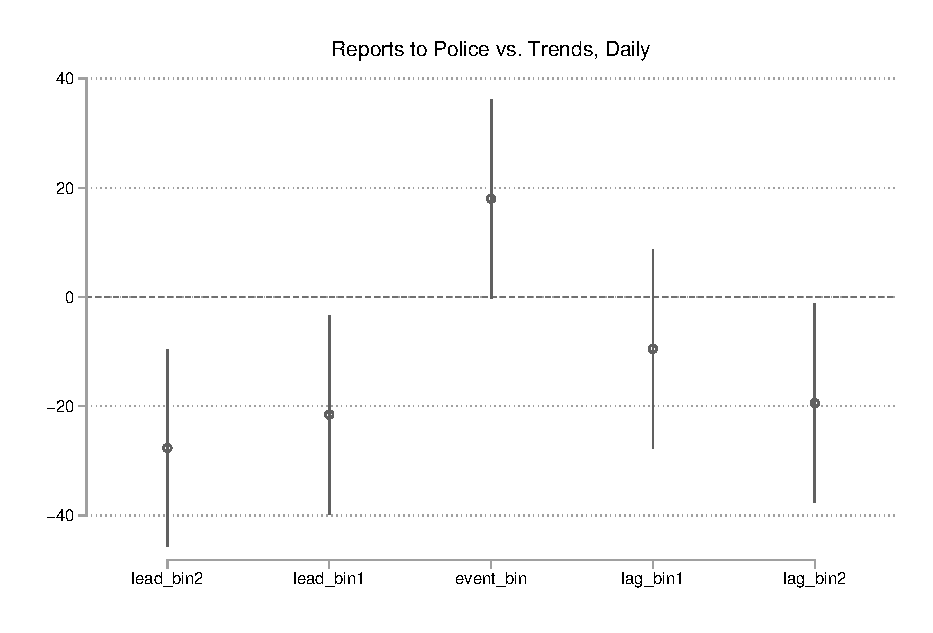
\includegraphics[width=\linewidth]{figures/events_police_binned_alle.eps}
\caption{Reports to the FBI before and after allegations of sexual assault}\label{figure:events_police_binned_alle}
\end{figure}

\begin{figure}
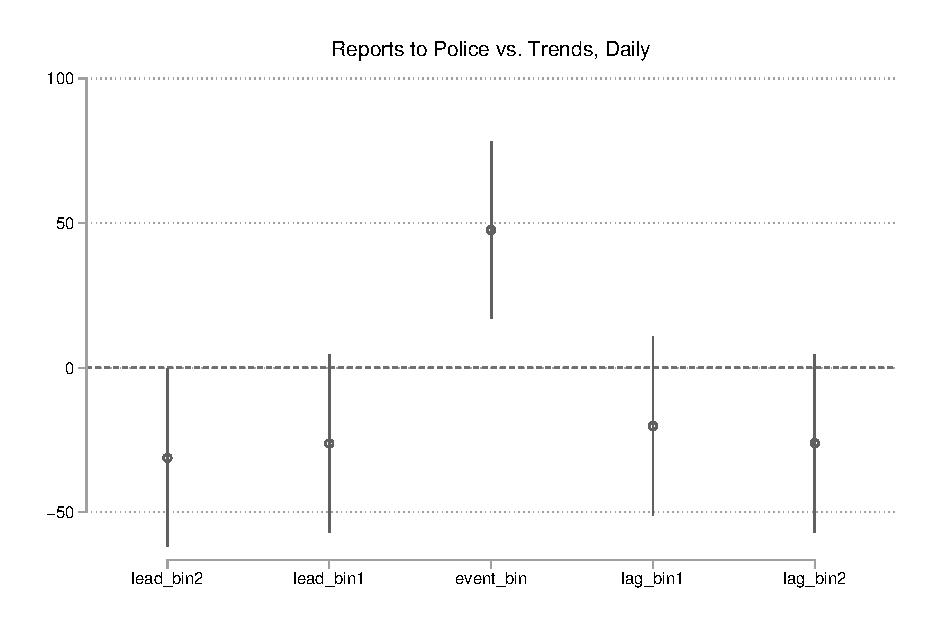
\includegraphics[width=\linewidth]{figures/events_police_binned_big.eps}
\caption{Reports to the FBI before and after 'Big Allegations'}\label{figure:events_police_binned_big}
\end{figure}

We see also see no significant individual days after allegations. After 'big allegations,' we see a large, statistically significant increase in reports 2 days after the event. 30 reports occuring that would otherwise not have after each of these high profile cases is huge. 

Here I think I want to bring up school reporting again. My narrative would go something like this:
\begin{itemize}
    \item Maybe we also see effects for much more local cases
    \item Potential evidencefor this: school reporting after title IX cases
    \item Show huge increase in reports at schools after title IX cases get opened there, explain that the cases are very salient as shown in \citeA{lindo_any_2018}
    \item However, looking closer this doesn't seem to hold up especially well
    \item Figure showing that effect is only on the first case, not subsequent ones
    \item Figures showing no increase in nearby schools or police stations (still need to rerun this, especially daily police) - maybe there is a small increase
\end{itemize}

\section{Discussion}

TBD

\clearpage
\section{To Discuss}

\begin{itemize}
    \item IDT analysis graph - hopefully. Otherwise methodology of it. Probably just qualitative. I'm found of using it as a way to discuss possible next steps.
    \item Talk about local/national T9 results with P Bayer. Bad news for my other results - other mechanisms? Although not the same type of event
    \item Talk about methodology on trend. Log? Original Trend?
    \item Best tables? Just one with overall effect, subgroups, columns are naive, instrument, log, log instrument? or something?
    \item Tables/Figures draft approx sequence
    \item Should make numbers national equivalent in tables? 
    \item Should I run with year interactions/something to check changing effect? Not that many years?
    \item IRF? Not sure I see what would be different than the graphs I have already
\end{itemize}


\clearpage 
\section{Next Steps}

\begin{itemize}
    \item Run state fixed effects with weights by population (once decided) as well as state cases
    \item Finish idt\_analysis. Graph
    \item Do same for 50/100/200 random generated time segments depending on time the above takes, compare shapes
    \item Check results on population1 - use if not ridiculous
    \item Calculate average event effect, equivalent to the US. Note the assumption in homogeneous effect.
    \item Find any more 
    \item Write a paragraph on future work. More on perpetrator behavior. More on whether increased reports are true new reports or just earlier reports.
    \item Put in methodology/somewhere about how this may be people reporting more quickly, not new reports. Assume some are new at least.
    \item Include state panel data with date fixed effects somewhere - null
    \item Look for more high-profile cases for event study. Go back before 2008, re-go-over already done dates
\end{itemize}


% The appendix command is issued once, prior to all appendices, if any.
\clearpage
%References here (manual or bibTeX). If you are using bibTeX, add your bib file 
%name in place of BibFile in the bibliography command.
% Remove or comment out the next two lines if you are not using bibtex.

\bibliographystyle{apacite}
\bibliography{refs}

\clearpage
\appendix

\chapter{High Profile Events}

\chapter{States included in FBI reporting}


\end{document}

